\section{Experimentacion}

Dedicamos este párrafo a describir las herramientas que usamos para experimentar en las próximas secciones. La herramienta que utilizamos para traducir el código de C++ a Assembler es \textit{objdump}, en base a esto podemos hacer comparaciones entre el código de C++ y Assembler. Para medir tiempos de compilación y ejecución utilizamos el comando \textit{time} y conservamos la medición de tiempo real, o sea, la correspondiente al tiempo que mide de un reloj de pared.

\colorbox{BurntOrange}{DUDA: Se va a analizar la memoria?}


\subsection{Análisis del código generado}

Usando la herramienta \textit{objdump} sobre los archivos objeto (.o) del código de C++ (sin flags de optimización), obtuvimos y analizamos el código ensamblado por el compilador. Notamos las siguientes caracterísicas del código generado que dan lugar a mejoras en el rendimiento:
\begin{itemize}
	\item Dentro de la función calcVelocities, la función donde se ralizan los cálculos que luego se vectorizarán, hay llamados a líneas consecutivas.
	\item Hay consultas a memorias innecesarias, por ejemplo, se pide un mismo valor a memoria varias veces, a pesar de haber sido guardado en un registro y nunca haber sido reemplazado con otro valor.
	\item Se manejan las variables locales almacenandolas en la pila, mientras que sólo se usan los registros de manera auxiliar para realizar operaciones.
\end{itemize}
Decidimos en consecuencia, analizar el mismo código de C++ aplicando algunas optimizaciones de compilador de GCC.

~\\

\subsection{Optimizaciones del compilador}


\subsubsection{Optimizaciones -O1}
El compilador de GCC posee una gran cantidad de optimizaciones. Un grupo de estas optimizaciones es habilitado por el parámetro -O1. Con el uso de esta optimización, el compilador se centra en reducir el tamaño del código y el tiempo de ejecución, a expensas de tiempo de compilación. Esto es comparando con la versión que no usa flags (-O0). Entre algunos de ellos se encuentran los siguientes flags:

\begin{itemize}
	\item \textit{fdce}: Realiza eliminación de código muerto en RTL \footnote{Register Transfer Language. Es una representación intermedia (RI), similar a Assembler. Se utiliza para describir el transferencia de datos de una arquitectura a nivel registro}, i.e. elimina instrucciones que no tienen efecto en la ejecución.
	\item \textit{fdse}: Realiza eliminación de guardado muerto en RTL, e.g. valores que son escritos a memoria de manera innecesaria.
	\item \textit{fsplit-wide-types}: Cuando se usa un tipo de datos que ocupa múltiples registros, como por ejemplo ``long long'' en un sistema de 32-bit, separa el dato y lo guarda de manera independiente. Esto, normalmente, genera mejor código para estos tipos de datos, pero hace más difícil el debuggeo.
	\item \textit{fmerge-constants}: Intenta unir constantes identicas (cadenas o flotantes) a través de unidades de compilación. Esta opción es la por defecto para la compilacion optimizada si el ensamblador y linker la soportan.
	\item \textit{fdelayed-branch}: No tiene efecto en el código pero causa la ejecución a priori en ramas de ejecución para aumentar la performance.
\end{itemize}

~\\

Analizamos los códigos generados por G++ con y sin flag de optimización -O1. Extrajimos la función \textit{set}, que implementa el seteo de un valor a la posición $(i, j)$ de una matriz y lo primero que notamos fue la diferencia en cantidad de las líneas de código.~\\
~\\
\center{\large{Función set de mat2}}
\begin{lstlisting}[]
  18e: 55                    push   rbp
  18f: 48 89 e5              mov    rbp,rsp
  192: 48 89 7d f8           mov    QWORD PTR [rbp-0x8],rdi
  196: 89 75 f4              mov    DWORD PTR [rbp-0xc],esi
  199: 89 55 f0              mov    DWORD PTR [rbp-0x10],edx
  19c: f3 0f 11 45 ec        movss  DWORD PTR [rbp-0x14],xmm0
  1a1: 48 8b 45 f8           mov    rax,QWORD PTR [rbp-0x8]
  1a5: 48 8b 10              mov    rdx,QWORD PTR [rax]
  1a8: 48 8b 45 f8           mov    rax,QWORD PTR [rbp-0x8]
  1ac: 8b 40 0c              mov    eax,DWORD PTR [rax+0xc] 
  1af: 0f af 45 f4           imul   eax,DWORD PTR [rbp-0xc]
  1b3: 89 c1                 mov    ecx,eax
  1b5: 8b 45 f0              mov    eax,DWORD PTR [rbp-0x10]
  1b8: 01 c8                 add    eax,ecx
  1ba: 48 98                 cdqe   
  1bc: 48 c1 e0 02           shl    rax,0x2
  1c0: 48 01 d0              add    rax,rdx
  1c3: f3 0f 10 45 ec        movss  xmm0,DWORD PTR [rbp-0x14]
  1c8: f3 0f 11 00           movss  DWORD PTR [rax],xmm0
  1cc: 90                    nop
  1cd: 5d                    pop    rbp
  1ce: c3                    ret    
  1cf: 90                    nop
\end{lstlisting}

La versión sin opitmizar, toma los parámetros cargados en registros, los guarda en la pila y luego vuelve a cargarlos a registros distintos. Incluso realiza accesos a memoria más de una vez en busca de un mismo dato.
En cambio, la versión del código de C++ mediante la optimización, utiliza los registros para el manejo de variables locales y accede solo las veces necesarias a memoria. Este es un claro ejemplo de los efectos de los flags \textit{fdse} y \textit{fdce}.


~\\~\\
~\\
\center{\large{Función set de mat2 con optimización -O1}}
\begin{lstlisting}[]
  d4: 0f af 77 0c           imul   esi,DWORD PTR [rdi+0xc]
  d8: 01 f2                 add    edx,esi
  da: 48 63 d2              movsxd rdx,edx
  dd: 48 8b 07              mov    rax,QWORD PTR [rdi]
  e0: f3 0f 11 04 90        movss  DWORD PTR [rax+rdx*4],xmm0
  e5: c3                    ret  
\end{lstlisting}




~\\

A pesar de las mejoras que notamos con el uso de la optimización, encontramos métodos donde no se eliminaban del todo los accesos innecesarios a memoria o los fragmentos de código sin utilidad. Tomamos otro extracto de código de la función \textit{calcVelocities} (donde se realizan los cálculos más complejos) y la analizamos. 

~\\
~\\
\center{\large{Función calcVelocities}}
\begin{lstlisting}[]
  1abe:	55                   	push   rbp
  1abf:	48 89 e5             	mov    rbp,rsp
  1ac2:	48 83 ec 38          	sub    rsp,0x38
  1ac6:	48 89 7d e8          	mov    QWORD PTR [rbp-0x18],rdi
  1aca:	89 75 e4             	mov    DWORD PTR [rbp-0x1c],esi
  1acd:	89 55 e0             	mov    DWORD PTR [rbp-0x20],edx
  1ad0:	48 8b 45 e8          	mov    rax,QWORD PTR [rbp-0x18]
  1ad4:	48 8d 88 e0 00 00 00 	lea    rcx,[rax+0xe0]
  1adb:	8b 55 e0             	mov    edx,DWORD PTR [rbp-0x20]
  1ade:	8b 45 e4             	mov    eax,DWORD PTR [rbp-0x1c]
  1ae1:	89 c6                	mov    esi,eax
  1ae3:	48 89 cf             	mov    rdi,rcx
  1ae6:	e8 00 00 00 00       	call   1aeb 
  1aeb:	f3 0f 11 45 d8       	movss  DWORD PTR [rbp-0x28],xmm0
  1af0:	48 8b 45 e8          	mov    rax,QWORD PTR [rbp-0x18]
  1af4:	48 8d 88 e0 00 00 00 	lea    rcx,[rax+0xe0]
  1afb:	8b 55 e0             	mov    edx,DWORD PTR [rbp-0x20]
  1afe:	8b 45 e4             	mov    eax,DWORD PTR [rbp-0x1c]
  1b01:	89 c6                	mov    esi,eax
  1b03:	48 89 cf             	mov    rdi,rcx
  1b06:	e8 00 00 00 00       	call   1b0b 
  ...     ...      ...        ...     ...
  2400:	f3 0f 10 45 d8       	movss  xmm0,DWORD PTR [rbp-0x28]
  2405:	89 c6                	mov    esi,eax
  2407:	e8 00 00 00 00       	call   240c 
  240c:	90                   	nop
  240d:	c9                   	leave  
  240e:	c3                   	ret    
  240f:	90                   	nop
\end{lstlisting}

La diferencia que notamos de los dos extractos de código de \textit{calcVelocities}, es el uso de la instrucción \textbf{nop}. El código de operación de \textbf{nop} corresponde a ``no operation'', no tiene ningun tipo de efecto, con lo cual, en el código optimizado se hace eliminación de este.
En la instrucción lad0 se carga el registro rax con un valor, no se lo pisa y luego vuelve a cargarlo en laf0. Este tipo de instrucciones donde no es necesario volver a cargar de memoria datos, vuelve a ser eliminado con el uso del flag fdse.

Volvemos a notar que en el código de C++ con flag -O1, el manejo de memoria no tiene el comportamiento de volver a cargar algo desde memoria que previamente había sido cargado y guardado en registros. Sin embargo, y apesar de las mejoras, vemos que aun repite movimientos de datos innecesarios entre registros.
Observando más detalladamente, el código con la mejora, no utiliza al máximo los registros, ya que guarda ciertos datos a memoria.
~\\
~\\
\center{\large{Función calcVelocities con optimización -O1}}
\begin{lstlisting}[]
  12f0:	41 57                	push   r15
  ...     ...                 ...    ...
  12f9:	53                   	push   rbx
  12fa:	48 83 ec 30          	sub    rsp,0x30
  12fe:	48 89 fb             	mov    rbx,rdi
  1301:	89 f5                	mov    ebp,esi
  1303:	41 89 d4             	mov    r12d,edx
  1306:	4c 8d bf e0 00 00 00 	lea    r15,[rdi+0xe0]
  130d:	4c 89 ff             	mov    rdi,r15
  1310:	e8 00 00 00 00       	call   1315
  1315:	0f 28 e0             	movaps xmm4,xmm0
  1318:	f3 0f 10 7b 1c       	movss  xmm7,DWORD PTR [rbx+0x1c]
  131d:	f3 0f 10 5b 14       	movss  xmm3,DWORD PTR [rbx+0x14]
  1322:	f3 0f 11 7c 24 04    	movss  DWORD PTR [rsp+0x4],xmm7
  1328:	0f 28 c7             	movaps xmm0,xmm7
  132b:	f3 0f 11 5c 24 10    	movss  DWORD PTR [rsp+0x10],xmm3
  1331:	f3 0f 5e c3          	divss  xmm0,xmm3
  1335:	0f 28 f0             	movaps xmm6,xmm0
  1338:	f3 0f 11 24 24       	movss  DWORD PTR [rsp],xmm4
  133d:	f3 0f 59 f4          	mulss  xmm6,xmm4
  1341:	f3 0f 11 74 24 08    	movss  DWORD PTR [rsp+0x8],xmm6
  1347:	8d 45 ff             	lea    eax,[rbp-0x1]
  134a:	44 89 e2             	mov    edx,r12d
  134d:	89 44 24 14          	mov    DWORD PTR [rsp+0x14],eax
  1351:	89 c6                	mov    esi,eax
  1353:	4c 89 ff             	mov    rdi,r15
  1356:	e8 00 00 00 00       	call   135b
  135b:	f3 0f 10 24 24       	movss  xmm4,DWORD PTR [rsp]
  ...       ...               ...     ...
  187a:	48 8d bb 30 01 00 00 	lea    rdi,[rbx+0x130]
  1881:	44 89 e2             	mov    edx,r12d
  1884:	89 ee                	mov    esi,ebp
  1886:	e8 00 00 00 00       	call   188b 
  188b:	48 83 c4 30          	add    rsp,0x30
  188f:	5b                   	pop    rbx
  ...   ...                   ...    ...
  1897:	41 5f                	pop    r15
  1899:	c3                   	ret 
\end{lstlisting}


~\\


Por último, analizamos los tiempos de ejecución del código de C++ con el flag de optimización -O1 y se obtuvieron los siguientes resultados en medición de tiempo de ejecución respecto al código sin flags de optimización:\\

\begin{center}
	\begin{tabular}{ccc}  
		\toprule 
		\multicolumn{2}{c}{Tiempo ejecución} \\
		\cmidrule(r){1-3}
		Tamaño & Sin optimización & Con optimización (O1)  \\
		\midrule
		6 x 6   &	8.328s 	&	3.260s	\\
		8 x 8	&	14.640s	&	5.776s	\\
		10 x 10	&	22.872s	&	8.980s	\\
		12 x 12 &	32.916s &   12.888s \\
		\bottomrule
	\end{tabular}\\
\end{center}

Los tiempos de ejecución se reducen utilizando el flag de optimización.\\
Por otro lado, los tiempos de compilación aumentan, como era esperado.

\begin{center}
  \begin{tabular}{cc}  
    \toprule 
    \multicolumn{2}{c}{Tiempo compilación} \\
    \cmidrule(r){1-2}
    Sin optimización & Con optimización (O1) \\
    \midrule
    0.652s  & 1.044s  \\
    \bottomrule
  \end{tabular}\\
\end{center}


  \colorbox{BurntOrange}{Esto puede volar e ir más adelante con el resto de las mediciones, lo dejo por las dudas}

~\\

%%%%%%%%%%%%%%%%%%%%%%%%%%%%%%%%%%%%%%%%%%%%%%%%%%%%%%%%%%%%%%%%%%%%%%%%%%%%%%%%%%%%%%%%%%%%%%%%%%%%%%%%%%%%%%%%%%%%%%%%%%%%%%%%%%%


\subsubsection{Optimizaciones O2}

Las optimizaciones de -O2 realizan mejoras de velocidad y tamaño de código tal que las mejoras de una no comprometan a la otra. En comparación con -O1, aumenta aún más el tiempo de compilación y la mejora de performace del código generado.Algunos de los flags que -O2 activa son:

\begin{itemize}
	\item \textit{falign-loops }:
	\item \textit{falign-labels}:
	\item \textit{fcaller-saves}:
	\item \textit{fcrossjumping}:
	\item \textit{fcse-follow-jumps}:
	\item \textit{fcse-skip-blocks}:
	\item \textit{fdelete-null-pointer-checks}:
	\item \textit{fdevirtualize}:
	\item \textit{fdevirtualize-speculatively}:
	\item \textit{fexpensive-optimizations}:

	\item \textit{fgcse}: Busca instancias de expresiones idénticas (i.e. que evaluan al mismo valor) y analiza si vale la pena reemplazarlas por una única variable reteniendo el valor computado\footnote{Common Subexpression Elimination (CSE).} de manera global. También realiza constant folding\footnote{Constant folding: Evaluar expresiones constantes en tiempo de compilación.} y constant propagation \footnote{Constant propagation: Sustitución de variables por sus valores constantes en expresiones en tiempo de compilación.}.
	
  \item \textit{fgcse-lm}: Intenta reordenar instrucciones donde se produzcan sucesivas cargas/guardados que pisan valores de una misma variable. Esto permite en los loops pasar de tener una variable (registro) que se carga constantemente, a una carga fuera del loop y copias y guardados en el loop.
	
  \item \textit{fhoist-adjacent-loads}:
	\item \textit{finline-small-functions}:
	\item \textit{findirect-inlining}:
	\item \textit{fipa-cp}:
	\item \textit{fipa-bit-cp}:
	\item \textit{fipa-vrp}:
	\item \textit{fipa-sra}:
	\item \textit{fipa-icf}:
	\item \textit{fisolate-erroneous-paths-dereference}:
	\item \textit{flra-remat}:
	\item \textit{foptimize-sibling-calls}:
	\item \textit{foptimize-strlen}:
	\item \textit{fpartial-inlining}:
	\item \textit{fpeephole2}:
	\item \textit{freorder-blocks-algorithm=stc}:
	\item \textit{freorder-blocks-and-partition}:
	\item \textit{freorder-functions}:
	\item \textit{frerun-cse-after-loop}:
	\item \textit{fsched-interblock}:
	\item \textit{fsched-spec}:
	\item \textit{fschedule-insns}:
	\item \textit{fschedule-insns2}:
	\item \textit{fstore-merging}:
	\item \textit{fstrict-aliasing}:
	\item \textit{ftree-builtin-call-dce}:
	\item \textit{ftree-switch-conversion}:
	\item \textit{ftree-tail-merge}:
	\item \textit{fcode-hoisting}:
	\item \textit{ftree-pre}:
	\item \textit{ftree-vrp}:
	\item \textit{fipa-ra}:
\end{itemize}

Notamos varios flags que aportan a la refactorización de código, que en consecuencia, ayudan a reducir el tamaño de código e incluso, con ayuda de los precálculos en tiempo de compilación, reducen tiempo de ejecución. 

Con lo cual, las instrucciones
~\\
~\\
\center{\large{Función setCavityFlowSpeeds con optimización -O1}}
\begin{lstlisting}[]
  106c:   83 7f 24 00             cmp    DWORD PTR [rdi+0x24],0x0
  1070:   7e 7d                   jle    10ef
  1072:   41 56                   push   r14
  1074:   41 55                   push   r13
  1076:   41 54                   push   r12
  1078:   55                      push   rbp
  1079:   53                      push   rbx
  107a:   48 89 fd                mov    rbp,rdi
  107d:   bb 00 00 00 00          mov    ebx,0x0
  1082:   4c 8d b7 b0 00 00 00    lea    r14,[rdi+0xb0]
  1089:   4c 8d af e0 00 00 00    lea    r13,[rdi+0xe0]
  1090:   4c 8d a7 10 01 00 00    lea    r12,[rdi+0x110]
  1097:   8b 45 28                mov    eax,DWORD PTR [rbp+0x28]
  109a:   8d 50 ff                lea    edx,[rax-0x1]
  109d:   f3 0f 10 05 00 00 00    movss  xmm0,DWORD PTR [rip+0x0]
  10a4:   00 
  10a5:   89 de                   mov    esi,ebx
  10a7:   4c 89 f7                mov    rdi,r14
  10aa:   e8 00 00 00 00          call   10af
  10af:   8b 45 28                mov    eax,DWORD PTR [rbp+0x28]
  10b2:   8d 50 ff                lea    edx,[rax-0x1]
  10b5:   f3 0f 10 05 00 00 00    movss  xmm0,DWORD PTR [rip+0x0] 
  10bc:   00 
  10bd:   89 de                   mov    esi,ebx
  10bf:   4c 89 ef                mov    rdi,r13
  10c2:   e8 00 00 00 00          call   10c7
  10c7:   8b 45 28                mov    eax,DWORD PTR [rbp+0x28]
  10ca:   8d 50 ff                lea    edx,[rax-0x1]
  10cd:   f3 0f 10 05 00 00 00    movss  xmm0,DWORD PTR [rip+0x0]
  10d4:   00 
  10d5:   89 de                   mov    esi,ebx
  10d7:   4c 89 e7                mov    rdi,r12
  10da:   e8 00 00 00 00          call   10df
  10df:   83 c3 01                add    ebx,0x1
  10e2:   39 5d 24                cmp    DWORD PTR [rbp+0x24],ebx
  10e5:   7f b0                   jg     1097
  10e7:   5b                      pop    rbx
  10e8:   5d                      pop    rbp
  10e9:   41 5c                   pop    r12
  10eb:   41 5d                   pop    r13
  10ed:   41 5e                   pop    r14
  10ef:   f3 c3                   repz ret 
  10f1:   90                      nop
\end{lstlisting}

~\\~\\
~\\
\center{\large{Función setCavityFlowSpeeds con optimización -O2}}
\begin{lstlisting}[]
  1880:   44 8b 5f 24             mov    r11d,DWORD PTR [rdi+0x24]
  1884:   45 85 db                test   r11d,r11d
  1887:   7e 72                   jle    18fb
  1889:   8b 47 28                mov    eax,DWORD PTR [rdi+0x28]
  188c:   4c 63 97 bc 00 00 00    movsxd r10,DWORD PTR [rdi+0xbc]
  1893:   31 d2                   xor    edx,edx
  1895:   4c 63 8f ec 00 00 00    movsxd r9,DWORD PTR [rdi+0xec]
  189c:   4c 63 87 1c 01 00 00    movsxd r8,DWORD PTR [rdi+0x11c]
  18a3:   83 e8 01                sub    eax,0x1
  18a6:   48 98                   cdqe   
  18a8:   49 c1 e2 02             shl    r10,0x2
  18ac:   48 c1 e0 02             shl    rax,0x2
  18b0:   49 c1 e1 02             shl    r9,0x2
  18b4:   49 c1 e0 02             shl    r8,0x2
  18b8:   48 89 c6                mov    rsi,rax
  18bb:   48 89 c1                mov    rcx,rax
  18be:   48 03 b7 b0 00 00 00    add    rsi,QWORD PTR [rdi+0xb0]
  18c5:   48 03 8f e0 00 00 00    add    rcx,QWORD PTR [rdi+0xe0]
  18cc:   48 03 87 10 01 00 00    add    rax,QWORD PTR [rdi+0x110]
  18d3:   0f 1f 44 00 00          nop    DWORD PTR [rax+rax*1+0x0]
  18d8:   83 c2 01                add    edx,0x1
  18db:   c7 06 0a d7 23 3c       mov    DWORD PTR [rsi],0x3c23d70a
  18e1:   c7 01 0a d7 23 3c       mov    DWORD PTR [rcx],0x3c23d70a
  18e7:   4c 01 d6                add    rsi,r10
  18ea:   c7 00 0a d7 23 3c       mov    DWORD PTR [rax],0x3c23d70a
  18f0:   4c 01 c9                add    rcx,r9
  18f3:   4c 01 c0                add    rax,r8
  18f6:   44 39 da                cmp    edx,r11d
  18f9:   75 dd                   jne    18d8
  18fb:   f3 c3                   repz ret 
  18fd:   90                      nop
  18fe:   66 90                   xchg   ax,ax
\end{lstlisting}

Analizaremos ahora las diferencias entre el codigo resultado de compilar con optimizaciónes -O1 y el que es generado por la compilación mediante optimizaciónes O2. Para eso tomaremos como objeto de estudio la función setCavityFlowSpeeds. Esta función es interesante ya que consiste de un unico ciclo, dentro del cual presenta un llamado a una función con una pequeña operatoria aritmetica. En particular lo que hace es recorrer el borde de cada matriz, y mediante un llamado a la función set, esta función concretamente multiplica el valor del indice i por el valor maximo que puede tomar la variable j y luego suma el valor de entrada de j a este resultado, abstrayendo asi el mecanismo de indexado en un arreglo plano.  
~\\
~\\
A grandes rasgos la optimización más notoria se constituye por un calculo previo al ciclado, de los distintos valores numéricos necesarios para luego acceder a las posiciónes de memoria necesarias. Este cálculo previo no se da en la versión -O1, sino que estos cálculos son realizados dentro del ciclo. Esto es claro ya que si observamos el ciclo que se constituye entre las lineas 1097 y 10e5 (24 instrucciónes) de la versión -O1, este consta de una mayor cantidad de líneas que el de la versión O2, 18d8, 18f9 (9 instrucciónes). Por el contrario, el código entre el inicio de la función y el del ciclo, es más largo en la versión O2. 
~\\
~\\


Además se puede notar la activación de los flags de alineamiento. Por ejemplo, se nota claramente la presencia de -falign-functions, que fuerza el comienzo de las funciónes en posiciones de memoria que sean multiplos de potencias de dos. Esto se logra insertando instrucciones sin efectos. Una forma de hacer esto es insertar líneas luego de un ret, que nunca se llegan a ejecutar. 

~\\
~\\

Si analizamos las direcciones de memoria donde se encuentran definidas las funciones, su último dígito siempre es cero. A continuación se muestran algunos ejemplos donde se ve el final de una función, con sus respectivas instrucciónes extra y el comienzo de la nueva función alineada.

~\\
calcVelocities:
\begin{lstlisting}[]
  1a99:   41 5d                   pop    r13
  1a9b:   41 5e                   pop    r14
  1a9d:   c3                      ret    
  1a9e:   66 90                   xchg   ax,ax

  1aa0 <_ZN9simulator14calcVelocitiesEii>:
  1aa0:   8b 8f ec 00 00 00       mov    ecx,DWORD PTR [rdi+0xec]
  1aa6:   41 57                   push   r15
  1aa8:   41 56                   push   r14
\end{lstlisting}
~\\
setPBorders:
\begin{lstlisting}[]
  18fb:   f3 c3                   repz ret 
  18fd:   90                      nop
  18fe:   66 90                   xchg   ax,ax

  1900 <_ZN9simulator11setPBordersEv>:
  1900:   41 56                   push   r14
  1902:   41 55                   push   r13
\end{lstlisting}

Se aclara que, la potencia de dos utilizada, es algo que se especifica en el flag cuando es utilizado por el usuario, y que no queda definida cuando este flag es agregado mediante el uso de -O2. Aún así el hecho de que el último dígito de todas las funciónes sea cero es un fuerte indicador de la presencia del efecto de esta optimización.\\
Comparamos dos versiones distintas del código de cpp con optimizaciones de -O1 (ambas) pero a una de ellas le agregamos el flag finline-small-functions, propia de las optmizaciones de O2. La finalidad de este experimento, es descubrir por qué razón hay funciones que hacen llamados a lineas consecutivas de su propio código.\\
Dichas llamadas en la versión con el flag finline-small-functions fueron reemplazadas por el código de las funciones utilizadas. Este es el caso de CavityFlowSpeeds, que hace uso de la función set. El código de muestra se puede ver aqui. (esta arriba. organizar)
\\
Al no encontrar una explicación clara sobre este comportamiento en el código, decidimos utilizar el siguiente comando g$++$ -4std$=$C$++$11 -DUSE\_CPP main.cpp  -S -masm$=$intel -o main.s para generar la versión de Assembler del código de cpp. Descubrimos que los raros llamados recursivos eran generados por \textit{objdump}.
\\

\colorbox{BurntOrange}{TODO: seguir redactando la experiencia esta y decimos que generamos con g++}

~\\
%%%%%%%%%%%%%%%%%%%%%%%%%%%%%%%%%%%%%%%%%%%%%%%%%%%%%%%%%%%%%%%%%%%%%%%%%%%%%%%%%%%%%%%%%%%%%%%%%%%%%%%%%%%%%%%%%%%%%%%%%%%%%%%%%%%


\subsubsection{Optimizaciones O3}

La optimización O3 mejora aún más los resultados, activa todas las optimizaciones de -O2 además de los siguientes flags:

\begin{itemize}
\item \textit{finline-functions}
\item \textit{funswitch-loops}
\item \textit{fpredictive-commoning}
\item \textit{fgcse-after-reload}
\item \textit{ftree-loop-vectorize}
\item \textit{ftree-loop-distribute-patterns}
\item \textit{ftree-slp-vectorize}
\item \textit{fvect-cost-model}
\item \textit{ftree-partial-pre}
\item \textit{fipa-cp-clone options}
\end{itemize}

La utilizacion del flag -O3 aumenta aun mas la cantidad de mejoras en busqueda del aumento d ela velocidad. La primera de ellas, finline-functions, es similar a su correspondiente flag en -O2, finline-small-functions, con la diferencia de que hace efecto sobre mayor cantidad de funciones, no limitandose solo a las funciónes mas pequeñas en cuanto a cantidad de codigo de cara a mantener baja la cantidad de lineas totales.
\\
En cuanto a funswitch-loops, no hay en el programa condiciones en ciclos que sean independientes de ellos ya que todos son función de las variables sobre las que se itera. La única instancia de esto que podria darse es en la condición que decide si utilizar Assembler o C++ plano pero esta no esta escrita en el lenguaje, sino que es una directiva del compilador.
\\
Tampoco se encuentran efectos de aplicar el flag fpredictive-commoning. De aplicar, el mismo ahorarría accesos a memoria guardando datos de una iteración de un ciclo para la siguiente. No se ven ahorros de accesos a memoria ni cambios en la forma en que se accede. Tampoco se ve ningun cambio en el codigo al incluir el flag en una compilación realizada con -O2 y realizar una diferencia entre este y el resultado de -O2 normal.




\subsection{Comparación entre secuencial, vectorial y multicore}
Ya analizado el tipo de mejoras que son implementadas por G++ al utilizar -O1, -O2 y -O3, se comparan mediciones de tiempo de los distintos flags presentes en el compilador, con otras formas de mejorar el rendimiento. En particular se estudia vectorización medinte SIMD y multicore mediante OpenMP.

Para cada mejora se experimentó con distintos tamaños del sistema simulado, yendo desde 1x1$m^2$ hasta 20x20$m^2$. Además, para cada tamaño, se realizaron 100 repticiónes, y se tomo la media y varianza de las mismas, con el objetivo de eliminar el error de medición introducido por la falta de control del tiempo otorgado a las distintas tareas del sistema operativo por parte del scheduler.

 
\begin{figure}[H]
\caption{Tiempo(s) vs Tamaño(m) para GCC}
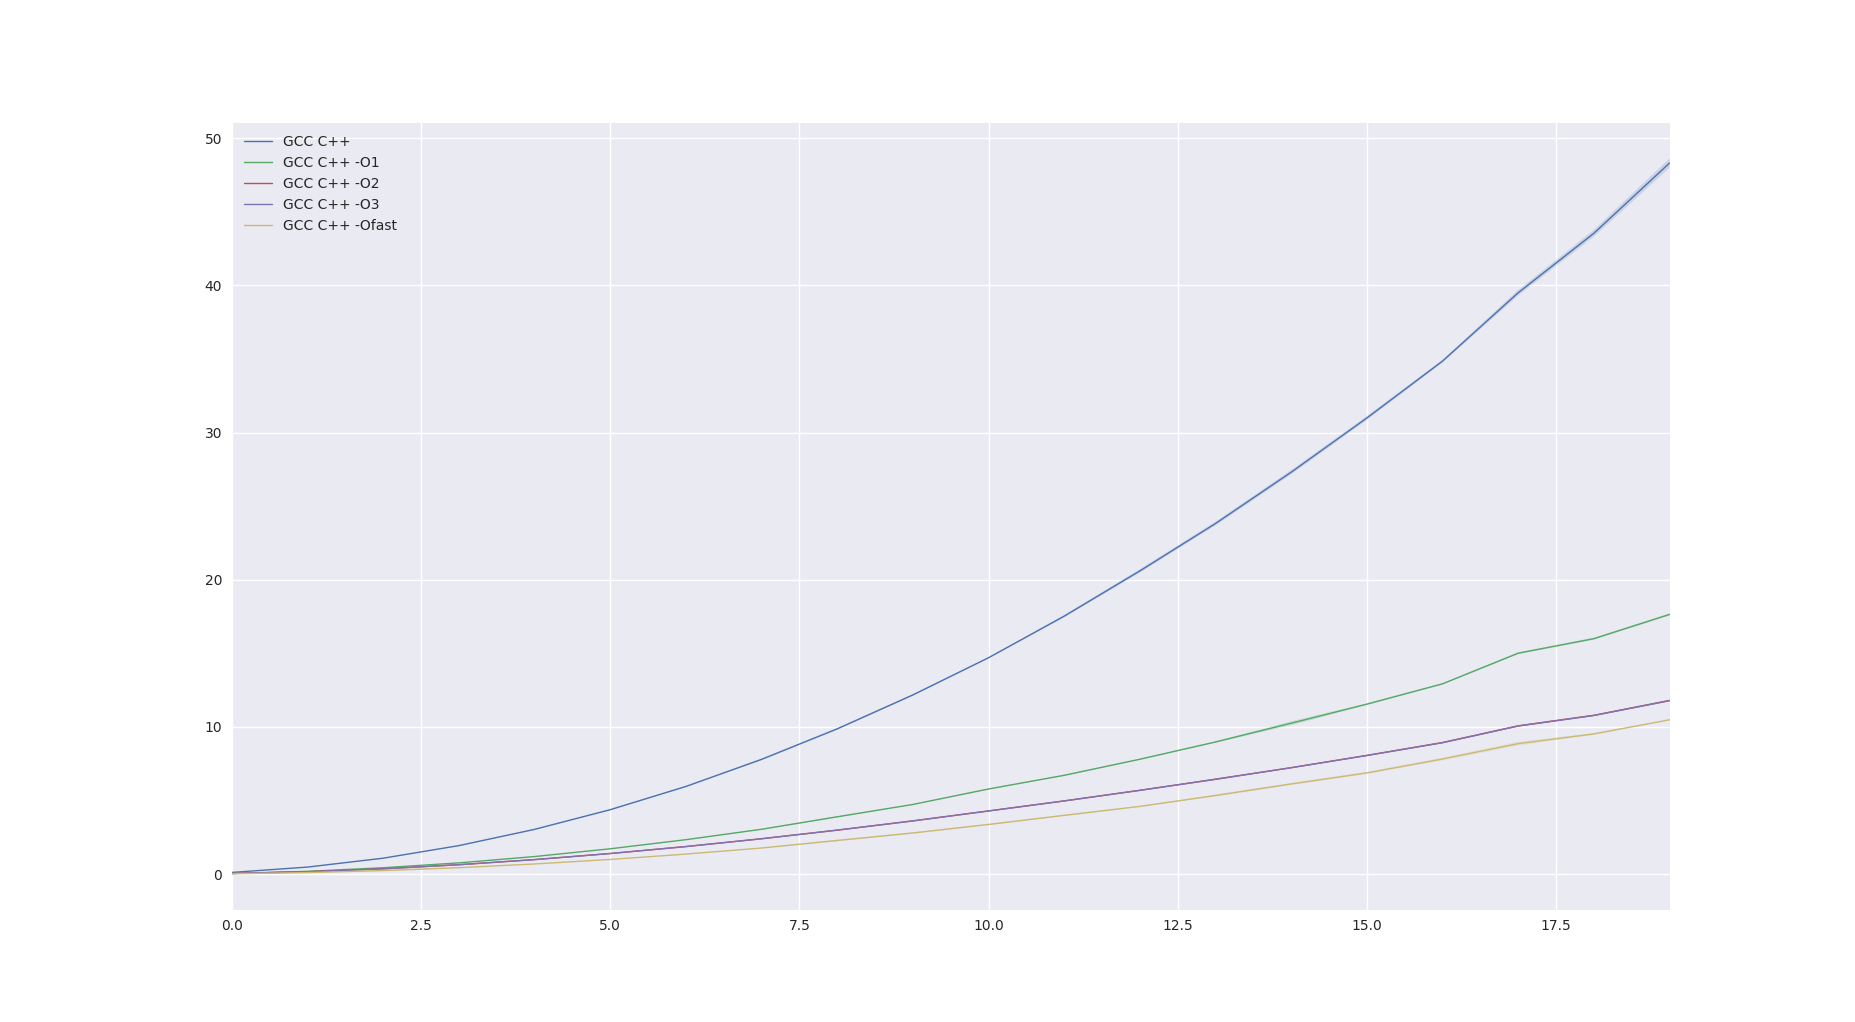
\includegraphics[width=\textwidth]{imagenes/plot_cpp.png}
\end{figure}

\begin{figure}[H]
\caption{Tiempo(s) vs Tamaño(m) para Intel C++ Compiler}
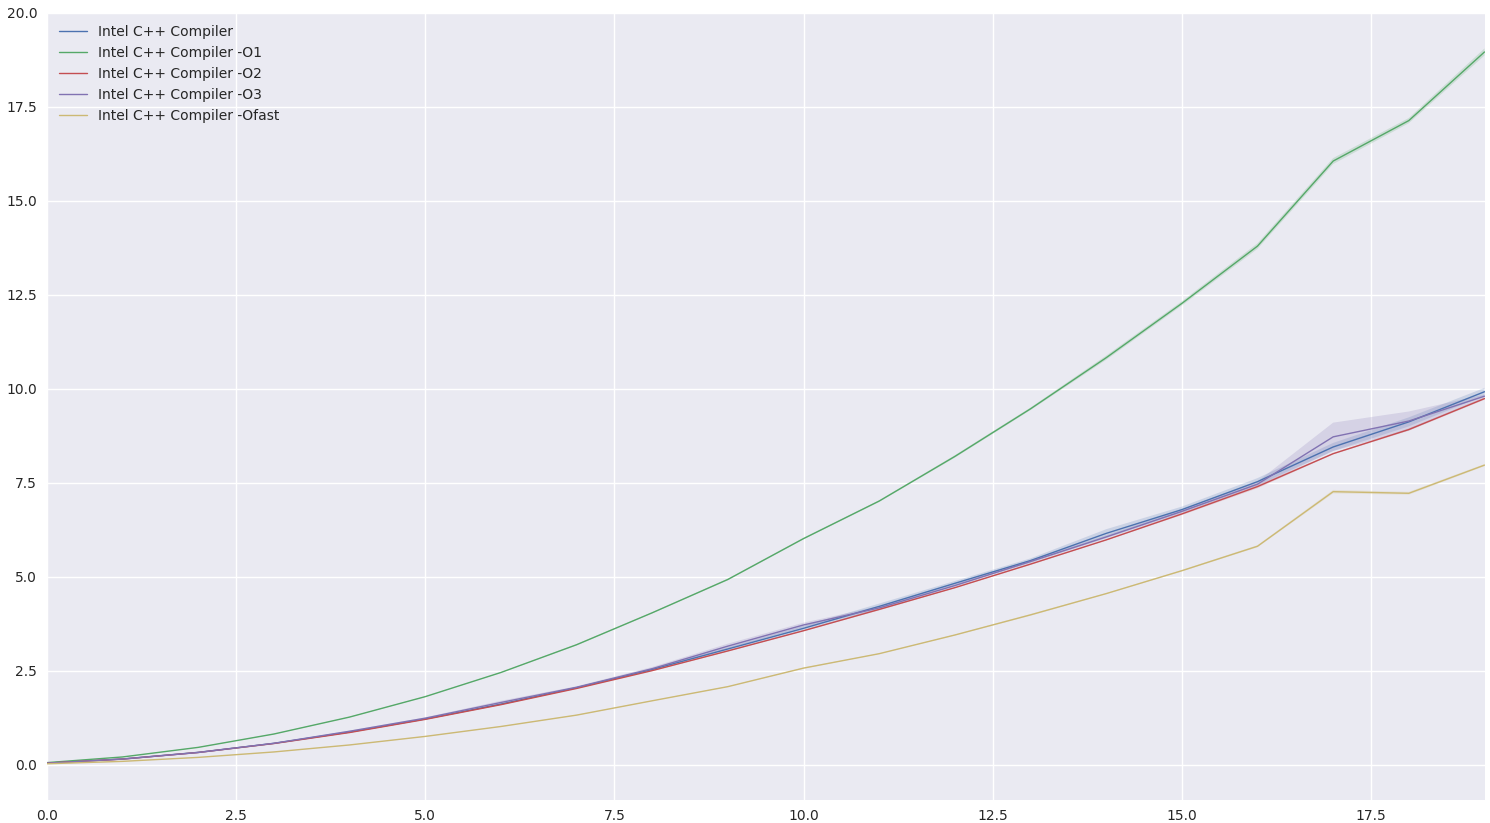
\includegraphics[width=\textwidth]{imagenes/plot_icc.png}
\end{figure}

\begin{figure}[H]
\caption{Tiempo(s) vs Tamaño(m) para Assembler(NASM)}
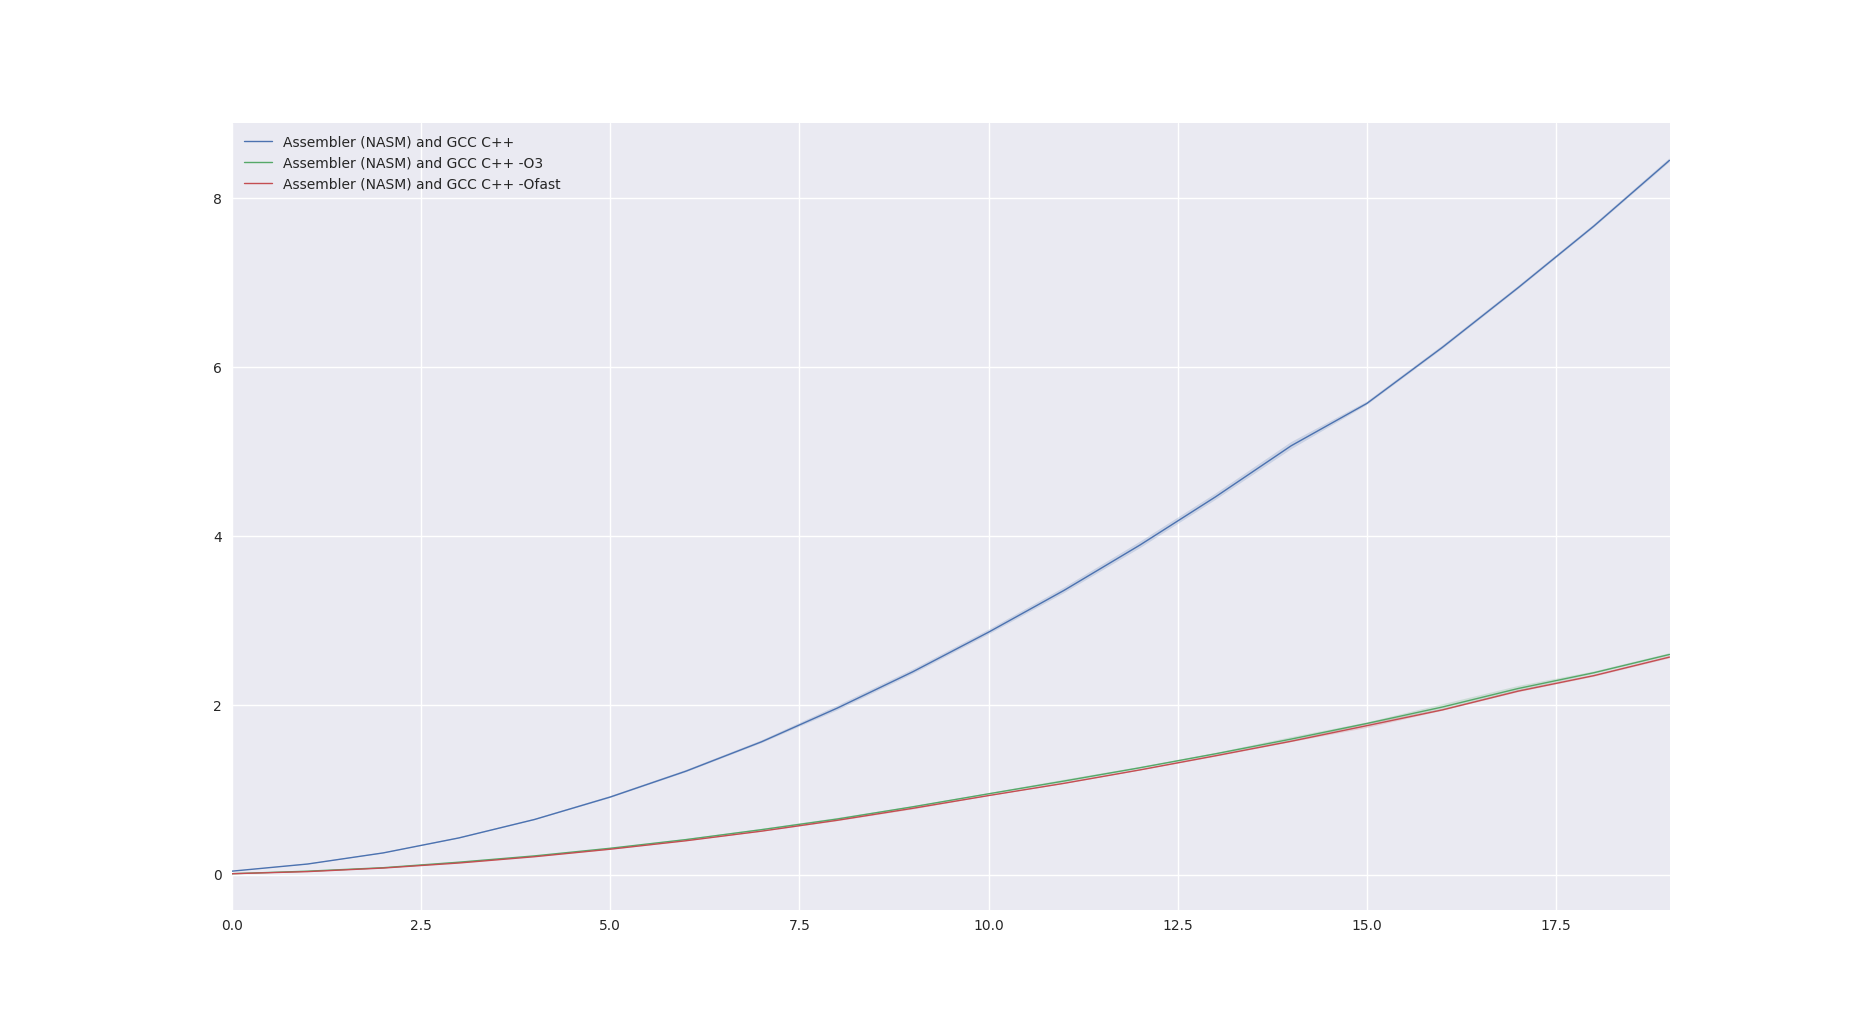
\includegraphics[width=\textwidth]{imagenes/plot_asm.png}
\end{figure}

\begin{figure}[H]
\caption{Tiempo(s) vs Tamaño(m) para GCC + OpenMP}
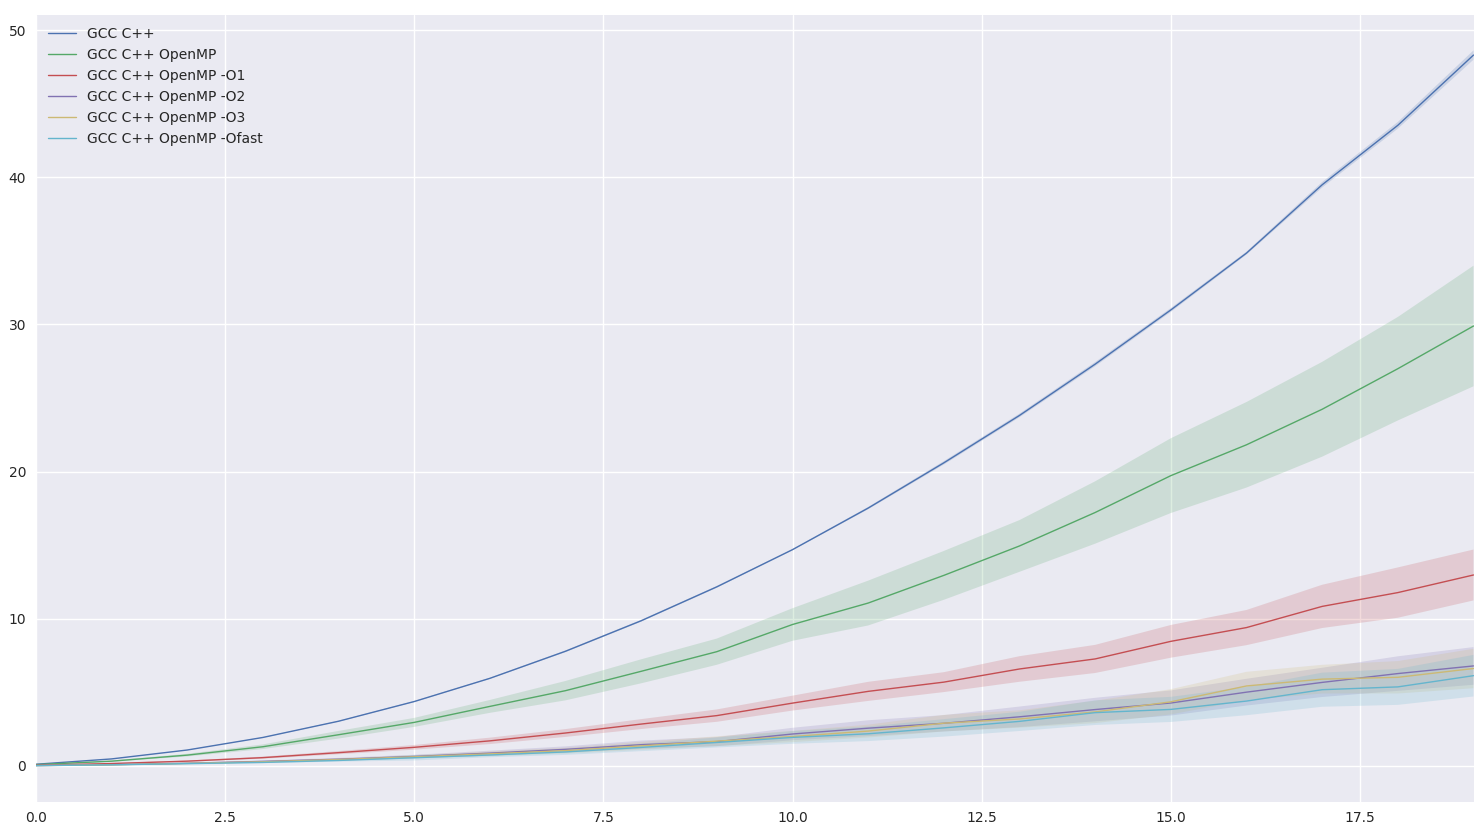
\includegraphics[width=\textwidth]{imagenes/plot_omp.png}
\end{figure}

\begin{figure}[H]
\caption{Tiempo(s) vs Tamaño(m) utilizando el flag -Ofast}
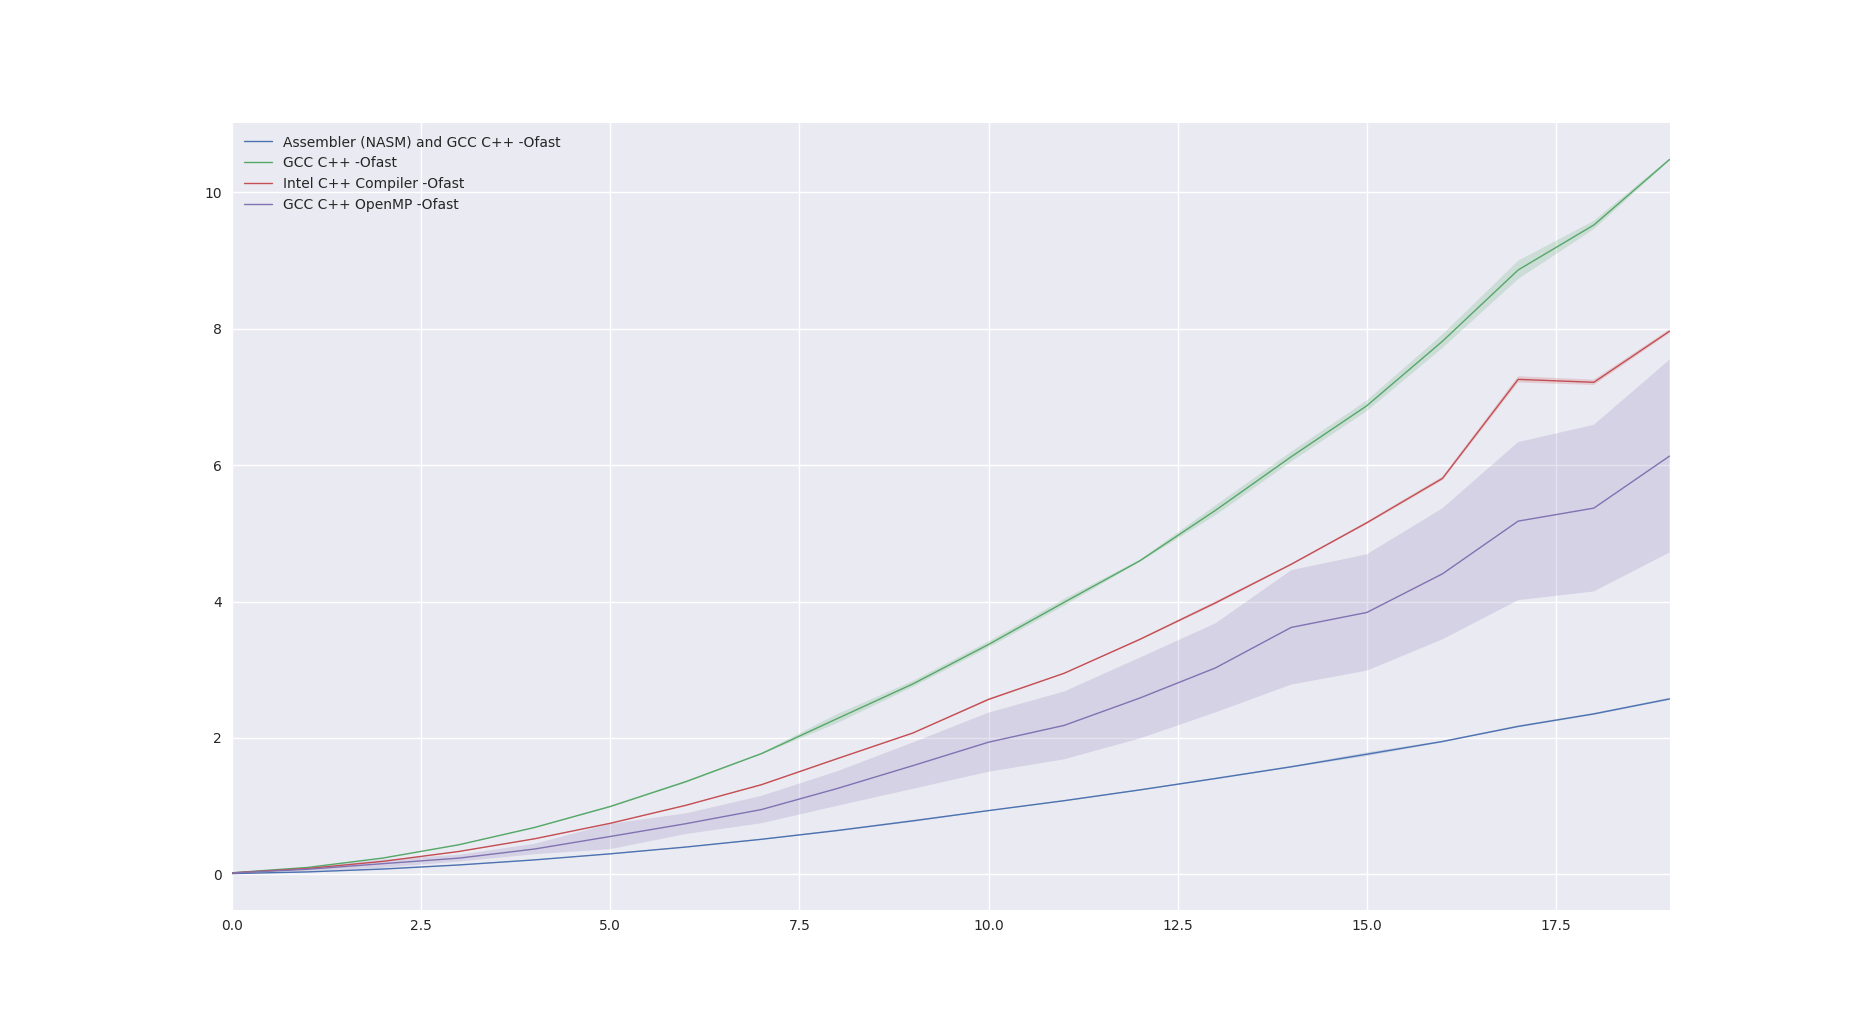
\includegraphics[width=\textwidth]{imagenes/plot_ofast.png}
\end{figure}

\begin{figure}[H]
\caption{Tiempo(s) vs Tamaño(m), todos los experimentos}
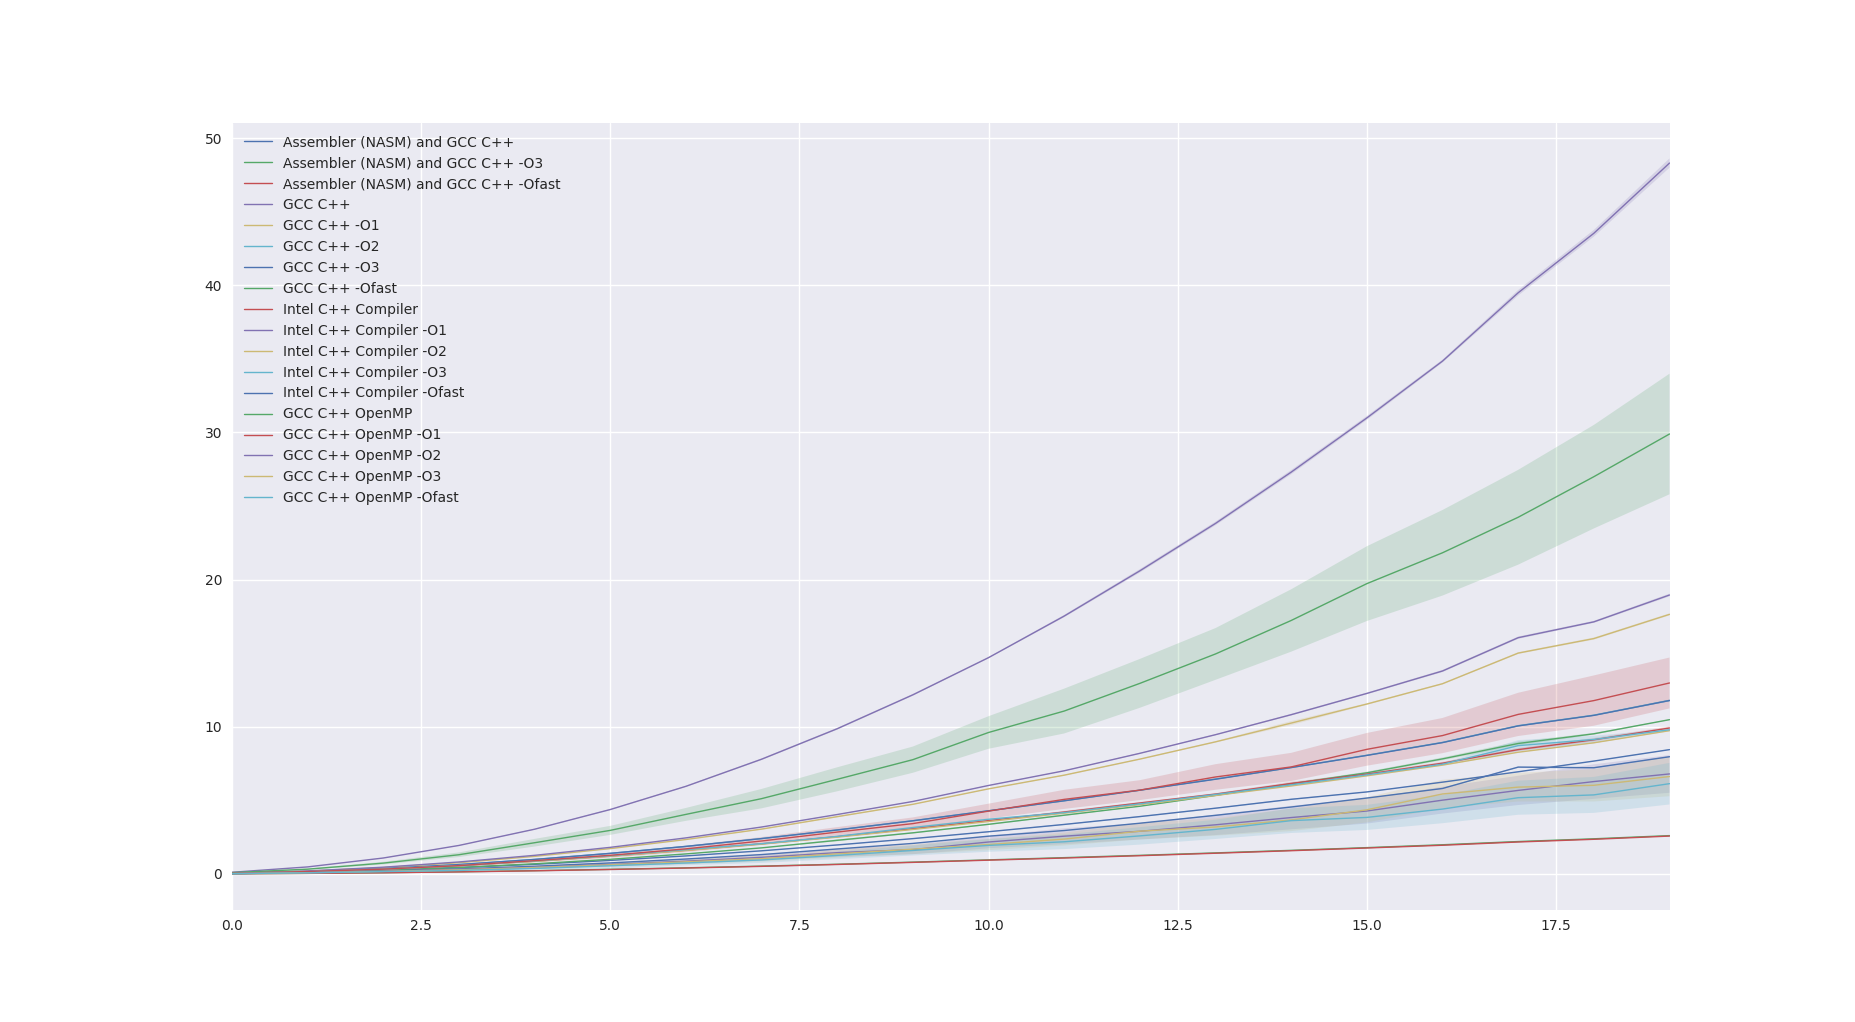
\includegraphics[width=\textwidth]{imagenes/plot_all.png}
\end{figure}


\subsection{CPU vs. memoria}

%con uderclock de la cpu o la ram